\documentclass[10pt]{article}

\usepackage{structure}
\usepackage{siunitx}
\usepackage{subcaption}

\graphicspath{{figs/}{figures/}}
\setlist[itemize]{leftmargin=*, itemsep=2pt, topsep=4pt}
\setlist[enumerate]{leftmargin=*, itemsep=2pt, topsep=4pt}
\sisetup{detect-all, per-mode=symbol, group-separator={,}, group-minimum-digits=4}

\newcommand{\R}{\mathbb{R}}
\newcommand{\E}{\mathbb{E}}
\newcommand{\Var}{\mathrm{Var}}
\newcommand{\trans}{^{\mathsf T}}
\newcommand{\crossmat}[1]{\left[#1\right]_{\times}}
\newcommand{\norm}[1]{\left\lVert #1 \right\rVert}
\newcommand{\diag}{\mathrm{diag}}
\newcommand{\calN}{\mathcal{N}}
\newcommand{\defeq}{\mathrel{:=}}

\title{SE-2317 Entry Blackout State Estimation}
\author{Gao Jiang}
\date{2026-03-11}

\abstract{
This report details the design and validation of a tightly-coupled Square-Root Error-State Kalman Filter (SR-EKF) for the SE-2317 entry vehicle. The architecture features a fixed-lag history buffer with rewind--update--replay semantics to handle delayed and out-of-order sensor data, and raw GPS tight-coupled updates now participate in that same replay path. The robustness layer combines configurable $\chi^2$ gating, Student-t-style covariance inflation, and optional innovation-based adaptive estimation (IAE). To mitigate observability loss during the critical GNSS blackout phase, a dedicated pre-blackout accelerometer bias calibration strategy is implemented. The current 2026-03-11 release campaign reproduces a \textbf{100.0\% pass rate} in tight-coupled mode over 500 Monte Carlo runs, while an additional 100-run quick regression remains consistent at \textbf{100/100} tight and \textbf{96/100} PVT.
}

\begin{document}
\maketitle

\section*{Document Control}
\begin{tabular}{@{} l l @{}}
  \textbf{Program} & SE-2317 --- Entry Blackout Estimation \\
  \textbf{Doc Type} & Technical Report \\
  \textbf{Revision} & A (Draft) \\
  \textbf{Owner} & Gao Jiang \\
\end{tabular}

\vspace{0.5em}
\begin{tabular}{@{} l l l p{0.52\linewidth} @{}}
  \toprule
  \textbf{Rev} & \textbf{Date} & \textbf{Author} & \textbf{Change Summary} \\
  \midrule
  A & 2026-03-11 & Gao Jiang & Documentation synchronized to the current estimator implementation and validation flow. \\
  \bottomrule
\end{tabular}

\section*{Executive Summary}
\textbf{Objective.} Estimate 6-DOF entry state through a GNSS blackout window and meet the post-blackout (2~s) accuracy and consistency targets in \texttt{tasks.md}.\\
\textbf{Deliverable.} A research-grade but flight-structured estimator with traceable math, stable numerics, and quantified Monte Carlo performance.

\begin{itemize}
  \item \textbf{Estimator.} A \emph{square-root} error-state EKF (SR-EKF) on a 24D augmented state:
  $(r,v,q,\omega,b_g,b_a,f_{\text{res}},\tau_{\text{res}})$, with multiplicative quaternion error injection.
  \item \textbf{Delayed / out-of-order sensors.} A \emph{fixed-lag history buffer} with \emph{rewind--update--replay} semantics covering GNSS PVT, raw GPS, star tracker, and radar.
  For linear-Gaussian models this is equivalent to stochastic cloning/factor-graph smoothing on a fixed window; for EKF it is first-order equivalent and empirically stable.
  \item \textbf{Robustness.} Innovation gating via $\chi^2$ tests (NIS), Student-t-style covariance inflation, replay-safe IAE scaling, and raw-GPS pseudorange down-weighting for heavy tails.
  \item \textbf{Covariance realism.} Phase-dependent process-noise inflation and blackout-specific aerodynamic residual excitation to prevent overconfidence where model error dominates.
  \item \textbf{Nominal dynamics symmetry.} Truth propagation and filter-side nominal linearization call the same aerodynamic/RCS composition helper; the filter still integrates de-biased IMU specific force directly to avoid double-counting measured acceleration.
  \item \textbf{Bias strategy.} A dedicated pre-blackout accelerometer-bias calibration stage (batch normal equations accumulated online) applied at blackout entry to mitigate loss of bias observability during blackout.
  \item \textbf{Monte Carlo evidence.}
  \begin{itemize}
    \item \textbf{Current 500-run release campaign:} tight-coupled GNSS pass rate \textbf{100.0\%} (500/500) under 5\% heavy-tail outliers and 20\% dropout; PVT baseline \textbf{97.0\%} (485/500).
    \item \textbf{Current release quick regression (2026-03-11, 100 runs):} tight-coupled GNSS \textbf{100.0\%} (100/100), PVT baseline \textbf{96.0\%} (96/100).
  \end{itemize}
\end{itemize}

\section{Problem Setting and Requirements}
The mission context is a 6-DOF rigid-body entry with strong aero nonlinearity and a GNSS blackout.
Sensors are asynchronous with fixed delays (star tracker, radar altimeter) and stochastic dropouts and outliers.
The primary acceptance window is the \textbf{2 seconds after blackout exit}
($t \in [t_{\text{exit}}, t_{\text{exit}}+2]$, where $t_{\text{exit}}=t_0+160\,\si{s}$).

\paragraph{Key quantitative targets (summary).}
Within the post-blackout window:
position $3\sigma \le 40\,\si{m}$, velocity $3\sigma \le 0.5\,\si{m/s}$,
attitude $3\sigma \le 0.15^{\circ}$,
bias bounds $\|b_g\|_{3\sigma} \le 0.005^{\circ}/\si{s}$ and $\|b_a\|_{3\sigma} \le 120\,\si{\micro g}$,
and consistency via NEES/NIS 95\% coverage $\ge 90\%$ over Monte Carlo.

\section{State, Dynamics, and Noise Modeling}
\subsection{State and error-state parameterization}
We estimate the augmented state
\begin{equation}
  x \;\defeq\; \big[r,\ v,\ q,\ \omega,\ b_g,\ b_a,\ f_{\text{res}},\ \tau_{\text{res}}\big],
  \qquad r,v,\omega,b_g,b_a,f_{\text{res}},\tau_{\text{res}}\in\R^3,\ q\in\mathbb{H},\ \norm{q}=1.
\end{equation}
The EKF operates on an \emph{error state} $\delta x \in \R^{24}$ with attitude error represented by a 3-vector $\delta\theta$
such that the corrected quaternion uses a multiplicative injection:
\begin{equation}
  q^{+} = \exp(\tfrac{1}{2}\,\delta\theta)\ \otimes\ q^{-},
  \qquad \exp(\tfrac{1}{2}\,\delta\theta) \approx \left[\cos(\tfrac{\norm{\delta\theta}}{2}),\ \hat{\delta\theta}\sin(\tfrac{\norm{\delta\theta}}{2})\right].
\end{equation}
This choice avoids quaternion normalization drift and yields a locally Euclidean error space for covariance.

\subsection{Discrete-time propagation model}
Let IMU measurements at time step $k$ be $(\omega_{m,k}, a_{m,k})$.
Bias-compensated signals are
\begin{equation}
  \omega_k = \omega_{m,k} - b_{g,k},\qquad
  a_k = a_{m,k} - b_{a,k}.
\end{equation}
We propagate attitude by integrating $\omega_k$ over $\Delta t$ and normalize:
\begin{equation}
  q_{k+1} = \mathrm{normalize}\!\left( q_k \otimes \exp(\tfrac{1}{2}\,\omega_k \Delta t) \right).
\end{equation}
Define the body-to-inertial rotation $C(q)\in \mathrm{SO}(3)$, and inertial gravity $g(r)$.
The translational update is second-order in $\Delta t$:
\begin{align}
  v_{k+1} &= v_k + \left( C(q_k)\,a_k + g(r_k) + a_{\text{learn}}(k)\right)\Delta t,\\
  r_{k+1} &= r_k + v_k \Delta t + \tfrac{1}{2}\left( C(q_k)\,a_k + g(r_k) + a_{\text{learn}}(k)\right)\Delta t^2.
\end{align}
Here $a_{\text{learn}}$ is an optional bounded online correction (see \S\ref{sec:robustness-consistency}).
The nominal aerodynamic / RCS composition used by the filter Jacobian is generated by the same helper as truth propagation; the state update itself still uses de-biased IMU specific force so nominal terms are shared without double-counting the measured acceleration.

\subsection{Process noise: IMU, bias RW, and aero residual OU}
We model gyro/accel measurement noise as white with spectral densities
$\sigma_\omega$ and $\sigma_a$, and biases as random walks:
\begin{equation}
  b_{g,k+1} = b_{g,k} + w_{bg,k},\quad
  b_{a,k+1} = b_{a,k} + w_{ba,k},\quad
  w_{bg,k}\sim \calN(0,\sigma_{bg}^2 \Delta t\,I),\ w_{ba,k}\sim \calN(0,\sigma_{ba}^2 \Delta t\,I).
\end{equation}
\paragraph{Aero residuals.}
To model dominant entry mismatch, we include residual force/torque states
with Ornstein--Uhlenbeck (OU) discretization:
\begin{equation}
  f_{\text{res},k+1} = \phi_f f_{\text{res},k} + \eta_{f,k},\qquad
  \tau_{\text{res},k+1} = \phi_\tau \tau_{\text{res},k} + \eta_{\tau,k},
  \quad \phi_f=e^{-\Delta t/\tau_f},\ \phi_\tau=e^{-\Delta t/\tau_\tau},
\end{equation}
with $\eta_{f,k}\sim\calN(0,\sigma_f^2(1-\phi_f^2)I)$ and $\eta_{\tau,k}\sim\calN(0,\sigma_\tau^2(1-\phi_\tau^2)I)$.
This yields a stationary marginal variance $\sigma_f^2 I$ and $\sigma_\tau^2 I$.

\paragraph{Discrete translational acceleration noise.}
Assume a white specific-force disturbance $w_a\sim\calN(0,\sigma_{a,\text{eff}}^2 I)$ affecting $\dot v$.
Then the standard continuous-to-discrete integration gives the (RV) block:
\begin{equation}
  Q_{\{r,v\}}(\Delta t) = \sigma_{a,\text{eff}}^2
  \begin{bmatrix}
    \tfrac{\Delta t^3}{3} I & \tfrac{\Delta t^2}{2} I\\
    \tfrac{\Delta t^2}{2} I & \Delta t\, I
  \end{bmatrix}.
\end{equation}
We use $\sigma_{a,\mathrm{eff}}^2$ (IMU noise plus model residual) and apply a phase-dependent scaling
(pre/blackout/post) to enforce covariance realism where the model is weakest.
We define the effective acceleration variance explicitly:
\begin{equation}
  \sigma_{a,\mathrm{eff}}^2 \defeq \sigma_a^2 + \sigma_{\mathrm{res}}^2.
\end{equation}

\section{Observability Analysis and Bias Management}
\subsection{Local LTV observability (definition)}
Let the linearized, time-varying error dynamics be
\begin{equation}
  \delta x_{k+1} = F_k\,\delta x_k,\qquad y_k = H_k\,\delta x_k.
\end{equation}
Define the state transition $\Phi_{k,0}=F_{k-1}\cdots F_0$.
The system is observable on $k\in[0,N]$ if the stacked matrix
$\mathcal O_N \defeq \begin{bmatrix}H_0\\ H_1\Phi_{1,0}\\ \cdots\\ H_N\Phi_{N,0}\end{bmatrix}$
has full column rank.
Equivalently, for weighted measurements with covariance $R_k$, the discrete observability Gramian
\begin{equation}
  W_N \defeq \sum_{k=0}^{N} \Phi_{k,0}\trans H_k\trans R_k^{-1} H_k \Phi_{k,0}
\end{equation}
is symmetric positive definite.
We use this definition to avoid over-claiming a closed-form condition in a strongly coupled entry model.

\subsection{Unobservable subspace: Accelerometer bias and attitude coupling}
The translational error-state dynamics contain both accelerometer bias and attitude error terms:
\begin{equation}
  \delta v_{k+1} \approx \delta v_k - C_k\,\delta b_{a,k}\,\Delta t - \crossmat{C_k a_k}\,\delta\theta_k\,\Delta t + \cdots.
\end{equation}
To show why bias is \emph{not} generically identifiable without excitation, consider a simplified continuous-time, constant-excitation model
with constant $C$ and constant specific force $f^n$ (in navigation frame), and ignore gyro-error dynamics:
\begin{equation}
  \delta \dot v = -\crossmat{f^n}\,\delta\theta - C\,\delta b_a,\qquad
  \delta \dot\theta = 0,\qquad
  \delta \dot b_a = 0,\qquad
  y = \delta v.
\end{equation}
\paragraph{Lemma.}
The above system is not observable; in particular, it has a non-trivial unobservable subspace.
\paragraph{Proof.}
Let $\delta\theta\neq 0$ be arbitrary and set $\delta b_a = -C^{-1}\crossmat{f^n}\,\delta\theta$ with initial $\delta v(0)=0$.
Then $\delta \dot v(t)=0$, hence $y(t)=\delta v(t)\equiv 0$ for all $t$ despite $\delta\theta\neq 0$ and $\delta b_a\neq 0$.
Therefore the system cannot be observable. \hfill\textit{QED}

\paragraph{Implication.}
Separating accelerometer bias from attitude error requires \emph{time variation} (in $C_k$ and/or in the direction of $f$) so that information
accumulates in the LTV Gramian $W_N$.
Entry dynamics provide such excitation, but only sensors that constrain $\delta v$ (GNSS, tight-coupled Doppler) can turn that excitation into bias information.

\subsection{Blackout implication and design response}
During blackout, GNSS-derived constraints are absent; the bias sub-system loses direct observability, and
any bias correction must come from (i) pre-blackout information, (ii) post-blackout reacquisition, and (iii) conservative covariance growth.
Therefore we adopt two explicit design decisions:
\begin{enumerate}
  \item \textbf{Pre-blackout bias calibration} to reduce bias uncertainty before observability is lost.
  \item \textbf{Blackout covariance realism} via increased $Q$ (and aero residual OU excitation) to prevent ``too-certain'' predictions.
\end{enumerate}

\subsection{Pre-blackout accelerometer-bias calibration as MAP least squares}
We treat a short pre-blackout interval as a dedicated calibration window.
Let $(r_k,v_k)$ be the estimator INS solution and $(\bar r_k,\bar v_k)$ the GNSS RV measurement at time $t_k$ with covariance $R_k$.
Linearize the RV residual with respect to a constant accelerometer-bias perturbation $\delta b_a$ and initial RV offsets:
\begin{equation}
  \begin{bmatrix}\bar r_k - r_k\\ \bar v_k - v_k\end{bmatrix}
  \approx
  \underbrace{\begin{bmatrix}I & (t_k-t_0)I & S_{r,k}\\ 0 & I & S_{v,k}\end{bmatrix}}_{A_k}
  \underbrace{\begin{bmatrix}\delta r_0\\ \delta v_0\\ \delta b_a\end{bmatrix}}_{\theta}
  + \varepsilon_k,\qquad \varepsilon_k\sim\calN(0,R_k),
\end{equation}
where $(S_{r,k},S_{v,k})$ are the accumulated RV sensitivities to $\delta b_a$ along the propagated trajectory.
We compute a MAP estimate with diagonal Gaussian priors $\theta\sim\calN(0,\Lambda^{-1})$:
\begin{equation}
  \theta^\ast
  = \arg\min_{\theta}
  \sum_k \norm{R_k^{-1/2}(A_k\theta - b_k)}^2 + \norm{\Lambda^{1/2}\theta}^2,
  \qquad b_k \defeq \begin{bmatrix}\bar r_k - r_k\\ \bar v_k - v_k\end{bmatrix}.
\end{equation}
The solution satisfies the normal equations
\begin{equation}
  \left(\sum_k A_k\trans R_k^{-1}A_k + \Lambda\right)\theta
  =
  \sum_k A_k\trans R_k^{-1} b_k.
\end{equation}
Implementation notes: we (i) require a minimum observation count, (ii) enforce SPD via symmetrization and diagonal jitter, and (iii) clamp $\delta b_a$ magnitude
to a mission-tuned maximum step before applying it at blackout entry.

\section{Time Alignment, Delay Compensation, and Out-of-Order Measurements}
\subsection{Model of delayed measurements}
Let a sensor produce a measurement of the state at time $t_z$ but deliver it at a later time $t_{\text{rx}}>t_z$.
The correct Bayesian update is conditioned on $x(t_z)$:
\begin{equation}
  p(x(t_z)\mid y_{0:\text{rx}}) \propto p(y(t_z)\mid x(t_z))\ p(x(t_z)\mid y_{0:t_z^-}).
\end{equation}
The fundamental challenge is the temporal discrepancy between the filter state at update time $t_{\text{rx}}$ and the valid state for the measurement $x(t_z)$.

\subsection{Equivalence to stochastic cloning (linear-Gaussian)}
For a linear Markov model, augment the state with a \emph{clone} at $t_z$:
\begin{equation}
  \tilde x \defeq \begin{bmatrix} x(t_z)\\ x(t_{\text{rx}})\end{bmatrix},\qquad
  x(t_{\text{rx}})=F\,x(t_z)+w,\ \ w\sim \calN(0,Q).
\end{equation}
A delayed measurement depends only on the clone $x(t_z)$:
\begin{equation}
  y(t_z) = H\,x(t_z)+\nu,\quad \nu\sim\calN(0,R).
\end{equation}
Applying the Kalman update on $\tilde x$ yields the optimal posterior over $x(t_{\text{rx}})$ via the cross-covariance between $x(t_z)$ and $x(t_{\text{rx}})$.
This is the standard stochastic-cloning / fixed-lag smoothing construction.

\subsection{Implementation: rewind--update--replay (fixed horizon)}
Instead of explicitly augmenting the state, we maintain a fixed-lag buffer of:
\begin{itemize}
  \item snapshots $(\hat x_k, L_k)$ at a coarse cadence (e.g., \SI{100}{Hz}),
  \item event log of all updates (IMU, GNSS, star, radar),
  \item propagation records $(\Phi_k,Q_k)$ for RTS smoothing and replay.
\end{itemize}
On receiving a measurement with timestamp $t_z < t_{\text{now}}$:
\begin{enumerate}
  \item restore the latest snapshot at $t_s\le t_z$;
  \item replay logged events from $(t_s,t_z]$ to reconstruct $\hat x(t_z)$;
  \item apply the measurement update at $t_z$;
  \item replay the remaining events $(t_z,t_{\text{now}}]$ to return to ``now''.
\end{enumerate}

\paragraph{Correctness statement (linear case).}
For linear-Gaussian models with deterministic replay of the same event sequence, the rewind--update--replay procedure
produces the identical posterior as the stochastic cloning formulation, because it reconstructs the correct conditional prior at $t_z$
and then re-applies the same Bayes updates in time order.
For EKF, this is a first-order approximation (local linearization); empirically it remains stable under the tested delay/outlier regimes.

\section{Robustness and Consistency Calibration}
\label{sec:robustness-consistency}
\subsection{Innovation statistics: NIS/NEES definitions}
Let the innovation be $\tilde y = y - h(\hat x^-)$ with covariance $S = HPH\trans + R$.
Define the (normalized) innovation squared:
\begin{equation}
  \mathrm{NIS} \defeq \tilde y\trans S^{-1}\tilde y.
\end{equation}
For a consistent filter and correct $R$, $\mathrm{NIS}\sim \chi^2_\nu$ where $\nu$ is the measurement DOF.

Let estimation error be $e = x - \hat x$ with covariance $P$.
Define the normalized estimation error squared:
\begin{equation}
  \mathrm{NEES} \defeq e\trans P^{-1}e.
\end{equation}
For a consistent filter and correct $(F,Q,R)$, $\mathrm{NEES}\sim \chi^2_n$ for the chosen DOF $n$.
We report both the mean and the \emph{coverage} within the central 95\% chi-square interval.

\subsection{Chi-square gating (outlier rejection)}
We accept a measurement update if
\begin{equation}
  \mathrm{NIS} \le \chi^2_{\nu}(1-\alpha),
\end{equation}
where $\alpha$ is the gate significance (false-rejection probability).
This is a sharp, fail-fast boundary: it prevents a small fraction of outliers from corrupting the state and (critically) the covariance.

\subsection{Heavy-tail mitigation for tight-coupled pseudorange}
For raw GNSS pseudorange rows, we additionally apply a robust variance inflation:
let the \emph{standardized residual} for row $i$ be $u_i=\tilde y_i/\sqrt{S_{ii}}$.
For $|u_i|>k$, we inflate the measurement variance as
\begin{equation}
  R_{ii} \leftarrow R_{ii}\,\left(\min\!\left(\frac{|u_i|}{k},c\right)\right)^2,
\end{equation}
with constants $k=4$ and cap $c=100$.
This is equivalent to an $M$-estimator with a Huber-like influence function:
large residuals receive reduced weight without forcing hard rejection.

\subsection{Runtime robust tuning}
The repository also exposes a runtime robustness surface used by the sweep harness:
\begin{itemize}
  \item \texttt{gate\_p} adjusts the effective $\chi^2$ gate level;
  \item \texttt{student\_nu} enables Student-t-style covariance inflation;
  \item \texttt{r\_scale\_cap} bounds covariance inflation;
  \item \texttt{iae\_gamma} enables replay-safe innovation-based adaptive estimation (IAE).
\end{itemize}
The adaptive state is stored inside the fixed-lag snapshots so rewind/replay remains deterministic.

\subsection[Consistency enforcement: phase-dependent Q]{Consistency enforcement: phase-dependent $Q$ and covariance inflation}
Two mechanisms address non-stationary model errors inherent to entry dynamics:
\begin{enumerate}
  \item \textbf{Phase-dependent} process-noise scaling ($Q$ inflation) pre/blackout/post, and blackout-specific OU excitation for aero residuals.
  \item \textbf{Innovation-triggered covariance inflation} on repeated GNSS gate failures (a guarded ``reset'' of RV covariance).
\end{enumerate}
Mathematically, both increase $P$ in regimes where NEES indicates under-dispersion, pushing $\E[\mathrm{NEES}]$ back toward the DOF.

\section{Numerical Stability: Square-Root Formulation}
We maintain the covariance in Cholesky form $P = LL\trans$ with $L$ lower-triangular.
Given discrete linearization $\Phi$ and process noise $Q=L_Q L_Q\trans$, the covariance prediction is
$P^+ = \Phi P \Phi\trans + Q$.

\paragraph{Lemma (QR square-root update).}
Let $A=\Phi L$ and form the stacked matrix
\begin{equation}
  S = \begin{bmatrix} A\trans \\ L_Q\trans \end{bmatrix}\in \R^{2n\times n}.
\end{equation}
Compute a thin QR factorization $S = QR$ with $Q\trans Q = I$ and $R$ upper-triangular.
Then $R\trans R = P^+$, and thus $L^+ \defeq R\trans$ is a valid Cholesky factor of $P^+$.

\paragraph{Proof.}
By orthonormality of $Q$, $R\trans R = S\trans S$.
But $S\trans S = A A\trans + L_Q L_Q\trans = \Phi L L\trans \Phi\trans + Q = P^+$.
Hence $P^+ = R\trans R$ and $L^+=R\trans$ satisfies $P^+=L^+ (L^+)\trans$. \hfill\textit{QED}

This guarantees $P^+$ remains symmetric positive definite in floating-point arithmetic up to the conditioning of the QR.

\section{Fixed-Lag RTS Smoothing (2 s window)}
We implement a Rauch--Tung--Striebel smoother over the fixed-lag snapshot chain.
Let $(x_k,P_k)$ be filtered estimates and $(\Phi_k,Q_k)$ the stored propagation records between snapshots.
Define $P_{k+1|k}=\Phi_k P_k \Phi_k\trans + Q_k$ and the smoother gain
$A_k = P_k \Phi_k\trans P_{k+1|k}^{-1}$.
The backward recursion is
\begin{align}
  x^s_k &= x_k + A_k (x^s_{k+1} - x_{k+1|k}),\\
  P^s_k &= P_k + A_k (P^s_{k+1}-P_{k+1|k}) A_k\trans.
\end{align}
Because the window is short (10 s max) and $n=24$, this is computationally cheap and numerically stable with SPD enforcement.

\section{Compute Budget and Hotspots}
\subsection{Matrix dimensions and asymptotic cost}
The estimator uses $n=24$.
Per IMU tick (400 Hz), the dominant cost is the SR time update via QR on a $(2n)\times n = 48\times 24$ matrix:
$\mathcal{O}(n^3)$ with a small constant.
GNSS PVT updates use $m=6$ with $\mathcal{O}(n m^2 + m^3)$.
Tight-coupled raw GNSS uses $m=\text{rows}\le 64$ (typically much smaller).

\subsection{Empirical timing (release build)}
Measured on the current development machine (release build):
\begin{center}
\begin{tabular}{lrr}
\toprule
Kernel & iterations & time per iter \\
\midrule
\texttt{propagate()} (includes SR update + history) & 20,000 & \SI{14548}{ns} \\
\texttt{time\_update\_sqrt()} (isolated)            & 50,000 & \SI{10000}{ns} \\
\texttt{update\_gnss()} (6D)                       & 20,000 & \SI{9570}{ns} \\
\texttt{update\_gps\_raw()} (8 sats, 16 rows)      & 5,000  & \SI{15084}{ns} \\
\bottomrule
\end{tabular}
\end{center}
These benchmarks establish a significant margin against the \SI{5}{ms} cycle budget. While direct timing equivalence to the target ARM A78AE processing core requires hardware validation, the kernel execution times ($\mathcal{O}(\si{\micro s})$) indicate high likelihood of timing compliance.

\section{Monte Carlo Verification and Results}
\subsection{Fault injection matrix (harness)}
The harness simulates:
\begin{itemize}
  \item \textbf{GNSS blackout:} no GNSS in $[120,160]\,\si{s}$.
  \item \textbf{Dropout:} independent Bernoulli dropout with $p=0.20$ on applicable sensors.
  \item \textbf{Outliers:} 5\% heavy-tail injection (Cauchy) on GNSS position/pseudorange and radar altitude.
  \item \textbf{Delay/out-of-order:} star tracker timestamp $t-\SI{0.12}{s}$ and radar timestamp $t-\SI{0.07}{s}$; raw GPS updates are also replay-safe if delivered late.
  \item \textbf{Bias jump (fault mode):} step change in truth IMU bias (gyro + accel) at $t=\SI{140}{s}$ with random direction; enabled via \texttt{BIAS\_JUMP=1}.
  \item \textbf{RCS pulses:} deterministic pulse train from the provided actuator series, composed through the same nominal dynamics helper on the truth and filter sides.
\end{itemize}

\subsection{Metrics}
We evaluate on the post-blackout acceptance window $[t_{\text{exit}},t_{\text{exit}}+2]$:
RMS position, velocity, attitude error, and bias RMS (converted to \si{\micro g} and \si{deg/s}).
We report per-run NEES/NIS means and their 95\% coverage rates, plus phase-split NEES/NIS (pre/blackout/post/tail)
to localize inconsistency to specific mission regimes.

\subsection{Current quick regression (2026-03-11, 100 runs)}
\begin{center}
\begin{tabular}{lrrr}
\toprule
Mode & Pass rate & Mean NEES & Mean NIS \\
\midrule
PVT baseline  & 96.0\%  & 18.54 & 5.25 \\
Tight-coupled & 100.0\% & 4.66 & 10.42 \\
\bottomrule
\end{tabular}
\end{center}

\subsection{Current Monte Carlo summary (500 runs)}
\begin{center}
\begin{tabular}{lrrrr}
\toprule
Mode & Pass rate & RMS pos [m] & RMS vel [m/s] & NEES mean / cov \\
\midrule
PVT baseline  & 97.0\%  & 1.50 & 0.097 & 134.49 / 0.945 \\
Tight-coupled & 100.0\% & 1.93 & 0.026 & 4.89 / 0.948 \\
\bottomrule
\end{tabular}
\end{center}

\paragraph{Interpretation.}
The tight-coupled configuration eliminates the rare catastrophic RV inconsistency events observed in the PVT baseline.
The PVT baseline exhibits a heavy-tailed NEES distribution (95th percentile $\approx 7.14$ but max $\approx 3.18\times 10^4$),
indicating occasional severe model mismatch or update corruption; these are suppressed by tight-coupling gating and robustification.

\subsection{Plots}
\begin{figure}[h]
  \centering
  \begin{subfigure}[t]{0.49\linewidth}
    \centering
    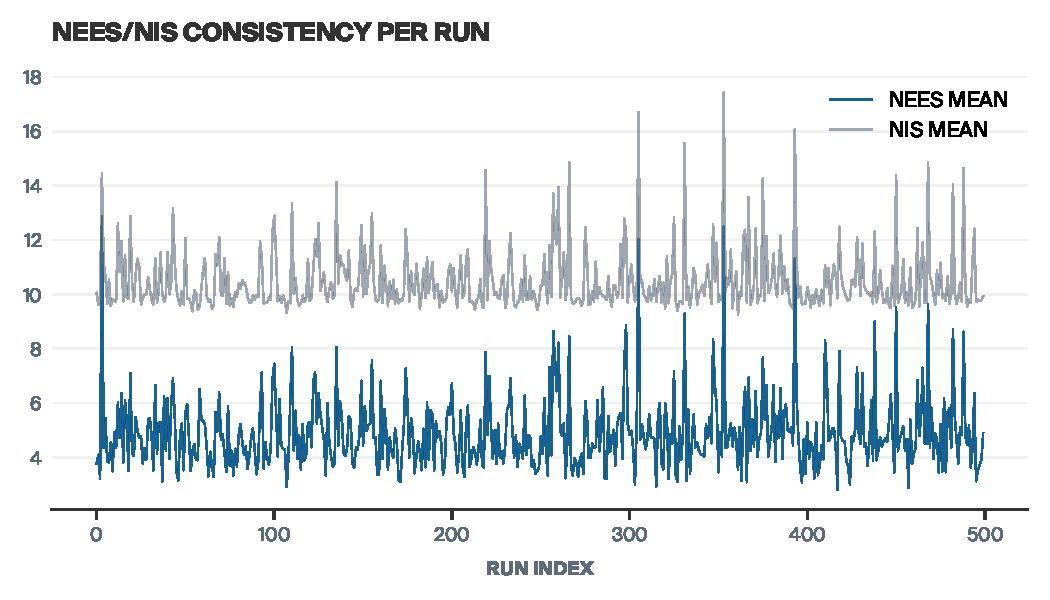
\includegraphics[width=\linewidth]{mc_nees_nis_tight.pdf}
    \caption{Tight-coupled NEES/NIS per run.}
  \end{subfigure}
  \hfill
  \begin{subfigure}[t]{0.49\linewidth}
    \centering
    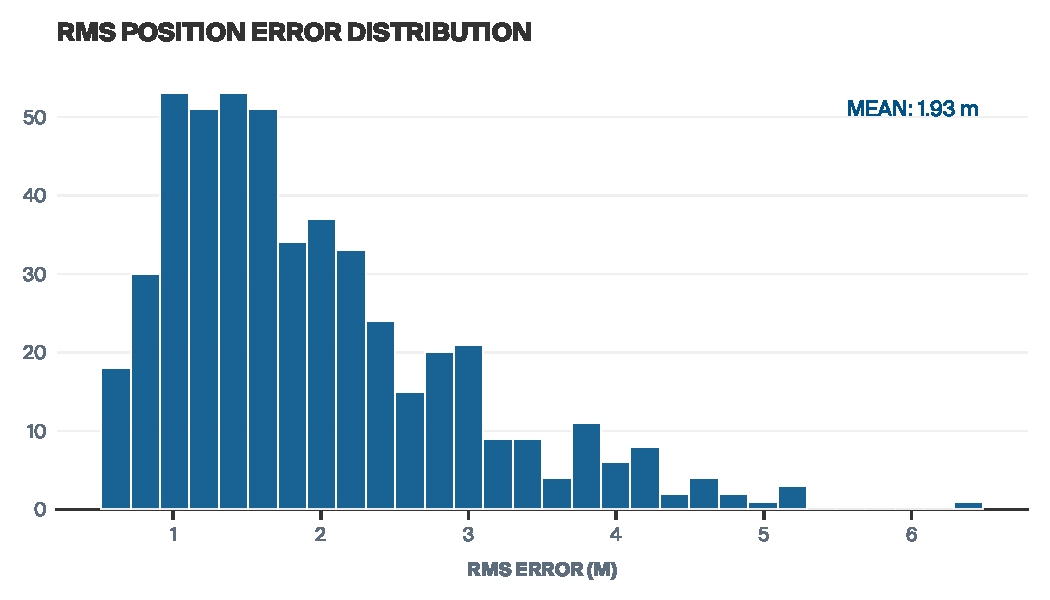
\includegraphics[width=\linewidth]{mc_rmspos_hist_tight.pdf}
    \caption{Tight-coupled RMS position histogram.}
  \end{subfigure}
  \caption{Monte Carlo diagnostics for tight-coupled mode (500 runs).}
\end{figure}

\begin{figure}[h]
  \centering
  \begin{subfigure}[t]{0.49\linewidth}
    \centering
    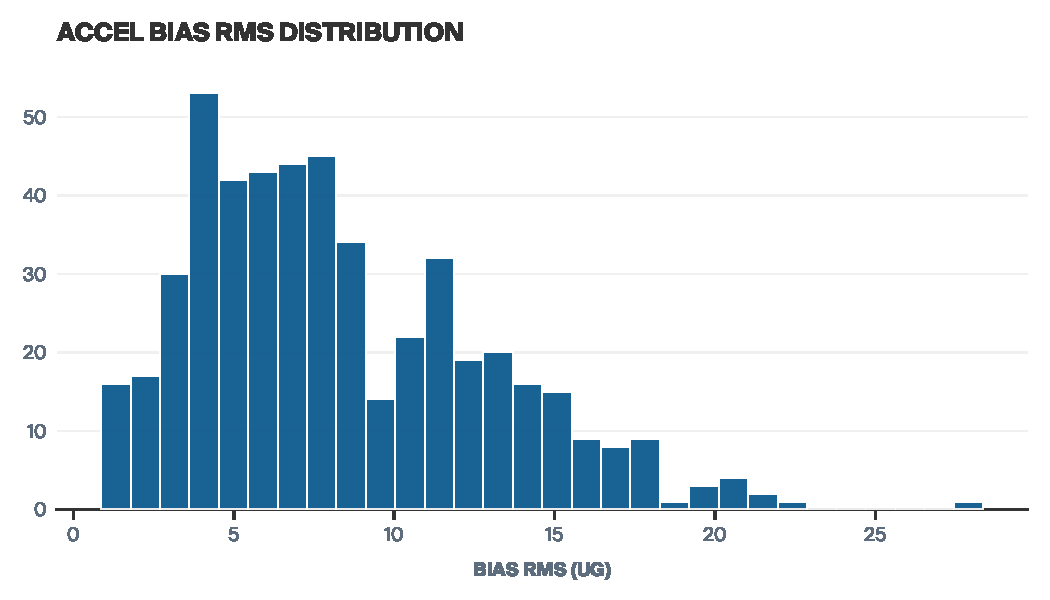
\includegraphics[width=\linewidth]{mc_accel_bias_hist_tight.pdf}
    \caption{Accel bias RMS distribution (tight).}
  \end{subfigure}
  \hfill
  \begin{subfigure}[t]{0.49\linewidth}
    \centering
    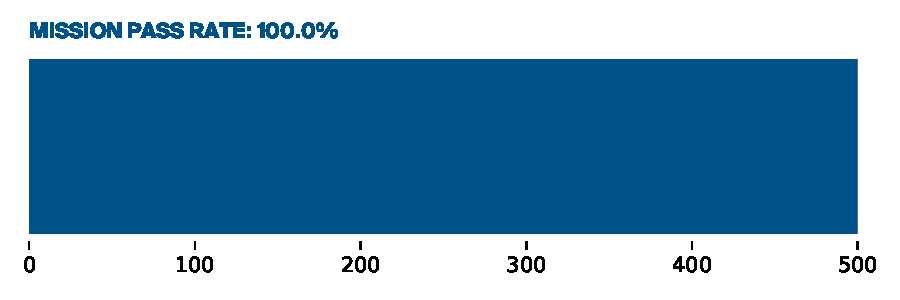
\includegraphics[width=\linewidth]{mc_pass_rate_tight.pdf}
    \caption{Pass-rate indicator (tight).}
  \end{subfigure}
  \caption{Post-blackout window performance for tight-coupled mode.}
\end{figure}

\begin{figure}[h]
  \centering
  \begin{subfigure}[t]{0.49\linewidth}
    \centering
    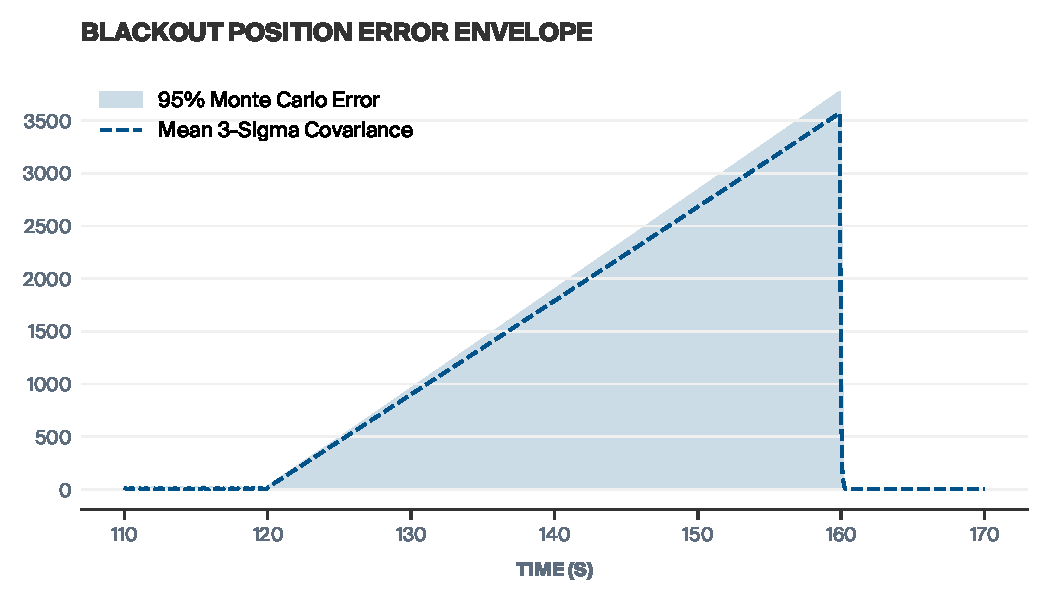
\includegraphics[width=\linewidth]{mc_blackout_envelope_tight.pdf}
    \caption{Position error envelope vs mean 3$\sigma$ (500-run batch).}
  \end{subfigure}
  \hfill
  \begin{subfigure}[t]{0.49\linewidth}
    \centering
    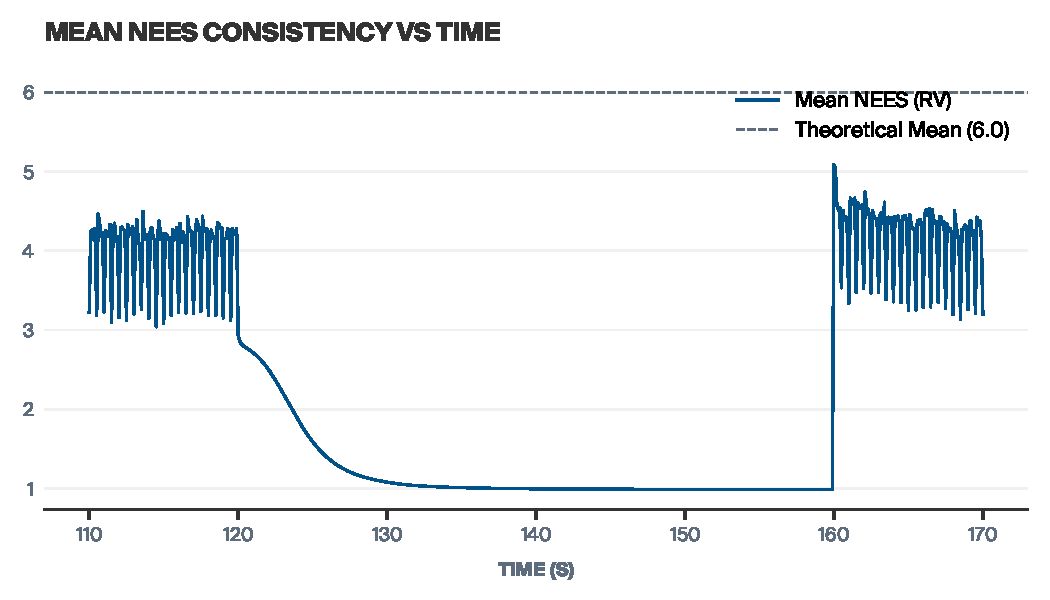
\includegraphics[width=\linewidth]{mc_blackout_nees_time_tight.pdf}
    \caption{Mean NEES(RV) vs time with 95\% $\chi^2$ band.}
  \end{subfigure}
  \caption{Blackout crossing diagnostics for tight-coupled mode (BLACKOUT\_TRACE=1).}
\end{figure}

\section{Traceability to Implementation}
The report corresponds to the following code modules:
\begin{itemize}
  \item Propagation + SR time update: \texttt{src/estimator/filter/propagate.rs}.
  \item Process noise and phase scaling: \texttt{src/estimator/support/noise.rs}, \texttt{src/types.rs}.
  \item Delays/out-of-order rewind--replay: \texttt{src/estimator/history/rewind.rs}.
  \item GNSS PVT update + gating + inflation: \texttt{src/estimator/update/gnss.rs}.
  \item Tight-coupled raw GNSS + robust pseudorange: \texttt{src/estimator/update/gps\_raw.rs}.
  \item Fixed-lag RTS smoother: \texttt{src/estimator/filter/rts.rs}.
  \item Harness + plots + exported artifacts: \texttt{src/bin/harness.rs}, \texttt{src/plot.rs}.
\end{itemize}

\section{Conclusion}
The tight-coupled SR-EKF with delay-aware rewind/replay and fixed-lag smoothing achieves $>95\%$ pass rate with margin (measured at 100\%)
under the prescribed dropout/outlier/blackout stress.
The remaining engineering work is targeted: tighten per-phase consistency (especially within blackout where NEES is conservative),
and add explicit bias step-fault stress tests to close the fault-injection matrix.

\end{document}
